\documentclass[a4paper]{article}

\usepackage[margin=2.5cm]{geometry}
\usepackage{fontspec}
% \usepackage[slantfont, boldfont]{xeCJK} % 允许斜体和粗体
\usepackage[UTF8]{ctex}

\setmainfont[Mapping=tex-text]{Liberation Serif} % 英文衬线字体
\setsansfont{Liberation Sans} % 英文无衬线字体
\setmonofont{Liberation Mono} % 英文等宽字体
\setCJKmonofont{Adobe Heiti Std} % 设置等宽字体
\setCJKsansfont{Adobe Song Std}
\setCJKmainfont{Adobe Song Std}

\punctstyle{kaiming} % 开明式标点格式
\usepackage{indentfirst} % 首段缩进
\setlength{\parindent}{2em}

\usepackage{xcolor}
\usepackage{graphicx}

\usepackage{mathrsfs}
\usepackage{bbding}

\usepackage{amsmath}
\usepackage{amsfonts}
\usepackage{amssymb}

\usepackage[xetex]{hyperref}
\hypersetup{colorlinks,
  linkcolor=black,
  filecolor=black,
  urlcolor=black,
  citecolor=black,
  pdftitle={AKS素性测试算法的证明m},
  pdfauthor={陈泓旭},
  pdfsubject={算法,素数判定},
  pdfkeywords={AKS primality testing},
  pdfproducer={xelatex} }

\usepackage{listings}
\usepackage{boxedminipage}
\usepackage{multicol}

\hfuzz=\maxdimen
\tolerance=10000
\hbadness=10000

\newtheorem{theorem}{定理}[section]
\newtheorem{lemma}{引理}[section]
\newtheorem{definition}{定义}[section]

\renewcommand{\abstractname}{摘要}
\renewcommand{\figurename}{图}
\renewcommand\refname{参考文献}

\numberwithin{equation}{section}

\title{AKS素性测试算法的证明}
\author{整理:陈泓旭\footnote{软件学院\quad 学号:1110379002}}
\date{}

\begin {document}
\maketitle
\begin{abstract}
  本文阐述了AKS素性测试( Primality Testing)算法的主要思想及具体证明过程;并和以往的素性测试算法进行了比较,指出了AKS算法在初等数论中的贡献。
\end{abstract}

\begin{multicols}{2}

  \section{引论}
  素数在理论数学界尤其是数论领域具有重要意义。相比于一般的自然数而言,素数有很多有趣的性质,素数性质的研究业已成为了初等数论的一个重要分支。如何高效地判
  定某个数是否为素数是一个基础而具有挑战性的问题。随着电子计算机技术和密码学的兴起,素数的判定测试显得更为重要。

  2002年8月6日,来自印度理工学院(IndianInstitute of Technology,IIT)的三位计算机科学家Manindra Agrawal, Neeraj Kayal和Nitin
  Saxen在论文\textit{``PRIMES is in P''}\cite{aks_paper} 中提出了AKS素性测试算法(也被称作Agrawal-Kayal-Saxena素性测试或分圆AKS测试),本文主要参考了这篇论文。该算法的重要之处在于它是一个同时具有一般性(gener
  al)、多项式复杂度(polynomial)、确定性(deterministic)和非条件性的(unconditional)的素性证明算法。
  \subsection{提出背景}
  质数,又称素数,指在一个大于1的自然数中,除了1和此整数自身外,无法被其他自然数整除的数(也可定义为只有1和本身两个因数的数)。

  素数的定义本身给定了判定素数的一个算法:\\[0.2cm]
  \begin{boxedminipage}{\columnwidth}\label{sieve}
    原始质数测试算法:\\
    输入:$n\in\mathcal{N},n>1$\\
    输出:当$n$是素数时返回$T$,否则返回$F$\\
    对所有满足$i\le\sqrt{n}$的数,判定$i$是否可以被$n$整除:\\
    如果存在这样的数$i$返回$F$,否则返回$T$
  \end{boxedminipage}


  该素性测试方法在古希腊早已有之,它是筛法求质数(Sieve of
  Eratosthenes)的一个特殊化。然而,对于一个素数$n$而言,判定是否为素数需要$\Omega (\sqrt
  n)$步。一般地,$n$占有$k=\Omega\log n$的位数,因此这需要$\Omega
  (2^\frac{k}{2})$,这样的算法时间复杂度是指数级的。然而一个高效算法的时间复杂度应当是多项式的($\lceil
  k\rceil$)。后来的数学家们曾经提出了很多素性测试方法,但都没有得到很好的效果。
  \subsection{理论基础}
  判定素性测试方法的好坏具有以下四个指标:
  \begin{enumerate}
  \item 普适性(general):判定素数的方法需要对所有的素数均成立。
  \item 多项式时间(polynomial):最大运行时间可用关于比特位的多项式函数刻画。
  \item 确定性(deterministic):判定方法需要准确指出是否为质数。
  \item 非条件性(unconditional):判定方法不应当基于任何尚未证明的假设。
  \end{enumerate}

  相比以往的素性判定算法,AKS算法很好地满足了上述四个条件。

  \section{预备知识}
  \subsection{\textit{P}和\textit{NP}问题}
  素数判定算法设计到复杂性理论中的一个重要概念:\textit{P}和\textit{NP}问题的判定。根据一个可解问题的时间复杂度,可以将问题分为\textit{P}和\textit{NP}问题。具体而言,涉及到下面几个
  概念:
  \begin{enumerate}
  \item \textbf{\textit{P}问题}\quad 所有可以由一个确定性图灵机在多项式表达的时间内解决的问题。
  \item \textbf{\textit{NP}问题}\quad
    所有可以在多项式时间内验证解是否正确的决定问题组成,等效地说,那些解可以在非确定型图灵机上在多项式时间内找出的问题的集合。
  \item \textbf{\textit{co-NP}问题}\quad
    一个问题$\mathcal{X}$是\textit{co-NP}的当且仅当它的补问题$\overline{\mathcal{X}}$是\textit{NP}问题。
  \item \textbf{\textit{NP-Complete}}\quad
    \textit{NPC}完全是一个复杂性问题类,这个问题类中的所有问题都是\textit{NP}问题,且类中各个元素(问题)可以相互规约。
  \item \textbf{\textit{NP-Hard}}\quad
    称一个问题\textit{H}是\textit{NP-Hard},当存在一个\textit{NPC}问题\textit{L}多项式图灵规约到它,即$L\le _T H$。
  \end{enumerate}

  显然,这几个集合之间并不是相互分离的。图\ref{fig:np} 给出了它们之间的关系。

  \begin{figure*}[htbp]
    \centering
    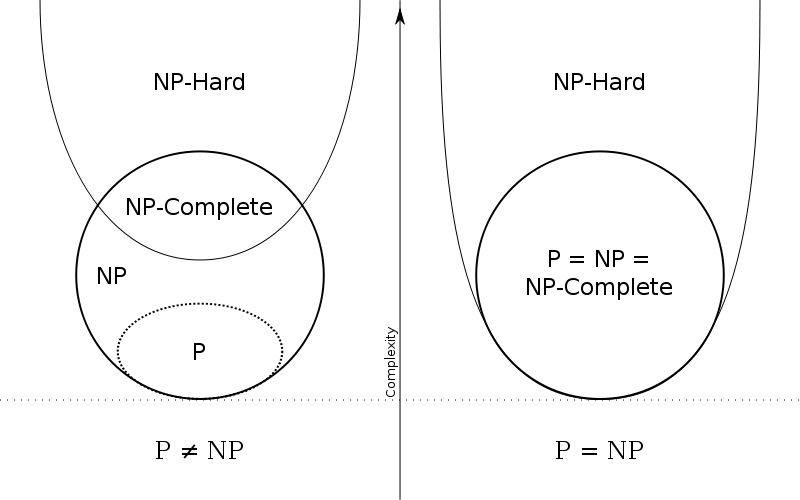
\includegraphics[width=\columnwidth]{fig/np}
    \caption{NP问题的Euler图}
    \label{fig:np}
  \end{figure*}

  \textnormal
  对于素性测试问题,可以看出它是\textit{co-NP}的,这是因为对于合数$n$,它必然有一个不为1和它本身的因子。1974年Pratt证明了该问题是\textit{NP}的\cite{aks}。而接下来
  使用的AKS算法证明,这个问题是$P$问题。
  \subsection{记号和术语}
  \noindent
  $\mathcal{Z}$ 整数集。\\
  $\mathcal{N}$ 自然数集。\\
  $\ln$ 以$e$为底的对数。\\
  $\log$ 以2为底的对数。\\
  $\mathit{Z}_n$ 整数在模$n$意义下形成的环。\\
  $F_p$ 含有$p$个元素的有限域,这里$p$是一个素数。\\
  $f(X)=g(X)\quad(\!\!\!\!\!\mod{h(X)},n)$:
  在环$\mathit{Z}_n\left[X\right]/(h(x))$上$f(X)=g(X)$。\\
  $O^{\sim}(t(n))$(其中$t(n)$是$n$的任意函数),等价于$O (t(n)poly(\log t(n)))$。\\
  给定$r\in \mathcal{N},a\in \mathcal{Z}$,$(a,r)=1$,$a$模$r$的阶是使得$a^k\equiv
  1\quad(\!\!\!\!\!\mod{r})$成立的最小正整数,记作$o_r (a)$。\\
  对于$r\in \mathcal{N}$,$\phi(r)$表示欧拉函数(Euler’s totient
  function),它表示小于$r$且和$r$互素的数的个数。容易看出,对于任意和$r$互素的$a$,有$o_r (a)|\phi(r)$。
  \subsection{一个不等式}
  \begin{lemma}\label{lcm}
    \upshape 令$LCM(m)$表示最先$m$个数的最小公倍数(least common
    multiple),则对于$m\ge 7$有
    \begin{equation}
      LCM(m)\ge 2^m
    \end{equation}
  \end{lemma}
  该定理的证明见\cite{nai82}。

  \section{主要思想}
  AKS算法主要是基于素数的下面这个特性,这一特性是费马小定理(Fermat’s Little
  Theorem)的一般化,它是\cite{AB03} 中随机多项式时间算法的基石。表述如下:
  % \paragraph{引理3.1}
  \begin{lemma}\label{idea}
    \upshape 令$a\in \mathcal{Z},n\in \mathcal{N},n\ge
    2$且$(a,n)=1$,则$n$是素数当且仅当
    \begin{equation}
      (X+a)^{n}\equiv X^n+a\mod{n}
    \end{equation}
  \end{lemma}
  \noindent \textbf{证明:}对$0<i<n$,在$((X+a)^n - (X^n +
  a))$中$x^i$的系数是$\binom{n}{i}\cdot a^{i-1}$.\\[0.2cm]
  假设$n$是素数,那么$n=0\mod{n}$因而所有的系数为0。\\[0.2cm]
  假定$n$是合数,考虑素数$q$使得它是$n$的一个因子,且使得$q^k||n$。则$q^k$不会整除$\binom{n}{q}$且和$a^{
    n-q}$不互素,因此$X^q$的系数不是$0\;(\!\!\!\!\!\mod{n})$.从而$((X+a)^n-(X^n+a))$在$\mathit{Z}_n$上不全为零。\P\\[0.2cm]
  上面模运算的一致性提供了一个素数的简单测试方法:给定一个输入值$n$,选择一个$a$并测试一致性是否满足。然而在最坏情形下我们需要计算$n$个系数,因此它的时间复杂
  度是$\Omega
  (n)$。可以采用一种简单的方法来减少数的数量:选取一个适当小的的$r$来计算上式两边对形如$X^r-1$的多项式取模的值,即我们可以通过测试下述等式是否成立来判定$n$是否是素数:
  \begin{equation}\label{key}
    (X+a)^n\equiv X^n+a \quad(\!\!\!\!\!\mod{X^r-1},n)
  \end{equation}

  从引理\ref{idea}立即可以看出所有的素数$n$对该式中任意$a$和$r$均满足。问题在于仍然存在合数$n$对于某些$a$和$r$也满足上面的式子。但我们可以确定
  的是,当适当选择$r$时,对一些$a$满足式子,则这样的$n$一定是素数。这样的$a$的数量和$r$的选取过程的时间复杂度都限于$\log
  n$,于是我们就得到了一个确定性的、多项式时间的素性测试算法。
  % ------------------------------------------------------------------------------
  \section{AKS算法}
  \subsection{核心算法}\label{sec_r1}
  \begin{boxedminipage}{\columnwidth}
    AKS算法\\
    输入:$n\in\mathcal{N},n>1$\\
    输出:当$n$是素数时返回$T$,否则返回$F$\\
    1.\quad 若 $n=a^b for a\in\mathcal{N} and b>1$,返回 $F$\\
    2.\quad 找到最小的$r$ s.t. $o_r (n)>\log^2 n$\\
    3.\quad 若对某个$a$,有$1<(a,n)<n$,返回$F$\\
    4.\quad 若$n\le r$,返回 $T$\\
    5.\quad 对$a\in\left[1\ldots\lfloor\sqrt{\phi (r)}\log n\rfloor\right]$若\\
    \indent\quad$\left((X+a)^n\ne X^n+a\;(\!\!\!\!\!\mod X^r-1,n)\right)$,返回$F$\\
    6.\quad 返回$T$
  \end{boxedminipage}
  \subsection{正确性证明}
  \begin{lemma}\label{pp}
    \upshape 当$n$是素数时,该算法返回值为$T$。
  \end{lemma}
  \textbf{证明:}若$n$为素数,则步骤1和3永远不会为真,由引理\ref{key} 可知,步骤5也不会返回。当满足$n\le
  r$时返回$T$;若不满足,则最终会返回$T$。$\P$\\[.2cm]
  反之,假设$n$在步骤4中返回$T$,则$n$必为素数。若不然,则步骤3中必能找到一个$n$的非1和本身的因子,必然会返回$F$。因此仅有的情况在于在步骤6中返回
  $T$。以下的分析均假设是这种情况。\\
  该算法有两个主要的步骤,即步骤2和步骤5。步骤2用于找一个合适的$r$,步骤5验证等式\ref{key}。

  首先需要找一个合适的$r$。
  \begin{lemma}
    \upshape 存在$r<\max\{3,\lceil\log^5 n\rceil\}$ s.t. $o_r (n)>\log^2 n$。
  \end{lemma}
  \textbf{证明:}{(\romannumeral 1)}结论对$n=2$的情况是平凡的,因为$r=3$对于所有情况均满足。\\
  {(\romannumeral 2)}当$n>2$时$\lceil\log^5 n>10\rceil$,则满足引理\ref{lcm}。注意到对于任何形如$m^k\le
  B,m\ge 2$的值有$k\le \lfloor\log B\rfloor$。现在考虑不能整除
  \begin{equation}
    n^{\lfloor\\log B \rfloor}\cdot \prod_{i=1}^{\lfloor\log^2 n\rfloor} (n^i-1)
  \end{equation}
  的最小整数$r$。值得注意的是$(r,n)$不可以被$r$的所有除数除尽,若不然则$r$必能被$n^{\lfloor\\log B
    \rfloor}$除尽。这样,$\frac{r}{(n,r)}$也不可被上式整除。而$r$是不能整除上式的最小的数,则有$(r,
  n)=1$。进一步,$r$不能整除满足$1\le i \le \lfloor \log^2 n \rfloor,o_r (n)>\log^2
  n$的$n^i-1$。从而有:
  \begin{equation}
    \begin{split}
      & n^{\lfloor\log B \rfloor}\cdot \prod_{i=1}^{\lfloor\log^2 n\rfloor} (n^i-1)\\
      < & n^{\lfloor\log B\rfloor + \frac{1}{2}\log^2 n\cdot (\log^2 n-1)}\\
      \le & n^{\log^4 n}\le 2^{\log^5 n}\le 2^B\\
    \end{split}
  \end{equation}
  由引理\ref{lcm} 得知开始$B$个数的最小公倍数至少为$2^B$,从而$r\le B$。\\
  由于$o_r (n)>1$则必存在一个为质数的除数$p$ s.t. $o_r
  (p)>1$。可以断言,$p>r$;否则的话测试必定能在步骤3或4中返回。这样,$(r,n)=1,p,n\in
  \mathcal{Z}_r^*$,于是可以确定$r$和$p$。令$\mathit{l}=\lfloor\sqrt{\phi (r)}\log n\rfloor$。
  步骤5验证用于验证等式$\mathit{l}$。由于在步骤5中不返回,则必有:
  \begin{equation}
    (X+a)^n\equiv X^n+a\;(\!\!\!\!\!\mod{X^r-1,n})
  \end{equation}
  对每个$a,0\le a\le \mathit{l}$都成立。这意味着:
  \begin{equation}
    (X+a)^n\equiv X^n+a\;(\!\!\!\!\!\mod{X^r-1,p})
  \end{equation}
  对所有$0\le a\le \mathit{l}$成立。由引理\ref{key} 得:
  \begin{equation}
    (X+a)^p\equiv X^p+a\;(\!\!\!\!\!\mod{X^r-1,p})
  \end{equation}
  对所有$0\le a\le \mathit{l}$成立。而由上述两个等式可得:
  \begin{equation}
    (X+a)^{\frac{n}{p}}\equiv X^{\frac{n}{p}}+a\;(\!\!\!\!\!\mod{X^r-1,p})
  \end{equation}
  对所有$0\le a\le \mathit{l}$成立。\\
  这样,$n$和$\frac{n}{p}$也具有类似质数$p$的性质。把它写成下面的性质:
  \begin{definition}
    \upshape 对于多项式$f(X)$及数$m\in\mathcal{N}$,称$m$对于$f(X)$是内省的(introspective)若
    \[\left[f(X)\right]^m\equiv f(X^m)\;(\!\!\!\!\!\mod{X^r,p}).\]
  \end{definition}
  于是$0\le a\le \mathit{l}$时,$n$和$\frac{n}{p}$对于$X+a$是内省的。下面的引理则说明对于乘法``内省数''是封闭的。
  \begin{lemma}\label{introspectiveN}
    \upshape 若$m$和$m^\prime$为$f(X)$的内省数,则$m\cdot m^\prime$也是。
  \end{lemma}
  \textbf{证明:}由$m$为$f(X)$的内省数,有
  \begin{equation}
    \left[f(X)\right]^{m\cdot m^\prime}\equiv\left[f(X^m)\right]^{m^\prime}\;(\!\!\!\!\!\mod{X^r,p}).
  \end{equation}
  由$m^\prime$为$f(X)$的内省数,则
  \begin{equation}
    \begin{split}
      \left[f(X^m)\right]^{m^\prime}&\equiv  f(X^{m\cdot m^\prime})\;(\!\!\!\!\!\mod{X^{m\cdot r},p})\\
      & \equiv f(X^{m\cdot m^\prime})\; (\!\!\!\!\!\mod{X^r,p})
    \end{split}
  \end{equation}
  综合,有
  \begin{equation}
    \left[f(X^m)\right]^{m^\prime}\equiv f(X^{m\cdot m^\prime})\;
    (\!\!\!\!\!\mod{X^r,p}).\P
  \end{equation}
  对于数$m$,当它在某个多项式下是内省的,则这个多项式的集合在乘法意义下也是封闭的:
  \begin{lemma}\label{introspectiveP}
    \upshape 若数$m$在$f(X)$和$g(X)$下是内省的,则它在$f(X)\cdot g(X)$下也是内省的。
  \end{lemma}
  \textbf{证明:}\[\left[f(X)\cdot g(X)\right]^m=\equiv\left[f(X)\right]^m\cdot\left[g(X)\right]^m\]
  \[\equiv f(X^m)\cdot g(X^m)\:(\!\!\!\!\!\mod{X^r-1,p}).\P\]

  引理\ref{introspectiveN},\ref{introspectiveP} 说明,集合$I=\{\left(\frac{n}{p}\right)^i\cdot p^j|i,j>0\}$
  对于集合$P=\{\prod_{a=0}^\mathit{l}\left(X+a\right)^{e_a}|e_a\ge 0\}$是内省的。\\[0.2cm]

  下面基于这两个集合我们定义两个群,这两个群将在证明中起到至关重要的作用。

  第一个群是所有在$I$中模$r$的数的余数。由于$(n,r)=(p,r)=1$,可知它是$\mathit{Z} _r^*$的一个子群。
  记该群为$G$且$|G|=t$,$G$由$n$和$p\mod{r}$生成;同时,由于$o_r(n)>\log^2 n,t>\log^2 n$。

  为了定义第二个群,我们需要一些在有限域上分圆多项式的知识。令$Q_r(X)$是$F_p$上的第$r$个分圆多项式。多项式$Q_r(X)$除以$X^r-1$并分解
  成不可再分的度为$o_r(p)$的因子。令$h(X)$是这样一个因子。由于$o_r(p)>1$,
  则$h(X)$的度大于1。第二个群就是$p$中所有模$h(X)$和$r$的多项式的余数的集合。
  记该集合为$\mathcal{G}$,这个群是域$F=h(X)/(h(X))$中的元素$X,X+1,X+2,\ldots,X+\mathit{l}$生成的,且它是$F$的加群的子集。\\[0.2cm]
  下述引理\ref{HLJ} 证明了$\mathit{G}$的大小的下界。
  \begin{lemma}[Hendrik Lenstra Jr]\label{HLJ}
    \upshape $|\mathcal{G}|\ge \binom{t+\mathit{l}}{t-1}$
  \end{lemma}
  \textbf{证明:}首先,$h(X)$是分圆多项式$Q_r(X)$的一个子式,$X$是$F$中的第$r$个本原单位根。现在说明,$P$中任意两个度小于$t$的不同的多项式将映
  射到$\mathcal{G}$中的不同元。
  令$f(X)$和$g(X)$是$P$中的这样两个多项式。假定在$F$中$f(X)=g(X)$,令$m\in
  I$,则有在$F$中$\left[f(X)\right]=\left[g(X)\right]
  $。由于$m$对于$f$和$g$都是内省的,且$h(X)$能整除$X^r-1$,则在$F$中:
  \begin{equation}
    f(X^m)=g(X^m)
  \end{equation}
  这意味着对于每一个$m\in\mathcal{G}$,$X^m$都是多项式$Q(Y)=f(Y)-g(Y)$的一个根。由于$(m,
  r)=1$,每一个这样的$X^m$都是第$r$个本原单位根。因此在$F$中有$|G|=t$个不同的$Q(Y)$的根。然而,由于$f,
  g$的选择可知它们的度小于$t$,矛盾!从而$f(X)\ne g(X)$。\\
  由于$\mathit{l}=\lceil\sqrt{\phi(r)}\log n\rceil<\sqrt{r}\log n<r$且$p>r$,对于$1\le
  i\ne j\le\mathit{l}$在$F_p$中有$i\ne
  j$。这样,在$F$中$X,X+1,X+2,\ldots,X+\mathit{l}$两两不等。另外,由于$h$的度大于1,对于满足$0\le a\le
  \mathit{l}$的所有$a$而言,在$F$中$X+a\ne 0$。
  因此$\mathcal{G}$至少存在$\mathit{l}+1$个度为1的不同的多项式。进一步,$\mathcal{G}$至少存在$\binom{
    t+\mathit{l}}{t-1}$个度小于$t$的不同的多项式。$\P$\\[0.2cm]
  下证$n$不是$p$的幂时,$|\mathcal{G}|$有上界:
  \begin{lemma}
    \upshape 若$n$不是$p$的幂,则$|\mathcal{G}|\le n^{\sqrt{t}}$。
  \end{lemma}
  \textbf{证明:}考虑下面的$I$的一个子集:
  \begin{equation}
    \hat{I}=\{\left(\frac{n}{p}\right)^i\cdot p^j\|0\le i,j\le
    \lceil\sqrt{t}\rceil\}
  \end{equation}
  若$n$不是$p$的幂,则$\hat{I}$中有$(\lfloor\sqrt{t}
  \rfloor+1)^2>t$个不同的数。而$|G|=t$,由抽屉原理,知$\hat{I}
  $中至少有两个值在模$r$的情况下相等。令$m_1<m_2$且$m_1\equiv m_2\!\!\!\!\!\mod{r}$,则我们有:
  \begin{equation}
    X^{m_1}\equiv X^{m_2}\!\!\!\mod{X^r-1}.
  \end{equation}
  令$f(X)\in P$,那么:
  \begin{equation}
    \begin{split}
      \left[f(X)\right]^{m_1}&\equiv f(X^{m_1})\:(\!\!\!\!\!\mod{X^r-1,p})\\
      &\equiv f(X^{m_2})\:(\!\!\!\!\!\mod{X^r-1,p})\\
      &\equiv\left[f(X)\right]^{m_2}\:(\!\!\!\!\!\mod{X^r-1,p})
    \end{split}
  \end{equation}
  即在$F$中有:
  \begin{equation}
    \left[f(X)\right]^{m_1}=\left[f(X)\right]^{m_2}
  \end{equation}
  因而,在$F$中$f(X)\in
  \mathcal{G}$是多项式$Q^\prime(Y)=Y^{m_1}-Y^{m_2}$的一个根。由于$f(X)$是$\mathcal{G}
  $的任意一个元素,于是可以断言在$F$中$Q^\prime(Y)$至少有$|\mathcal{G}|$个根。
  而$Q^{\prime}(Y)$的度为$m_1\le \left(\frac{n}{p}\cdot
    p\right)^{\lfloor\sqrt{t}\rfloor}\le n^{\sqrt{t}}$,这表明$\mathcal{G}\le
  n^{\sqrt{t}}$。\P
  \begin{lemma}
    \upshape 若AKS算法返回$T$则$n$是素数。
  \end{lemma}
  \textbf{证明:}假设AKS算法返回$T$,引理\ref{HLJ} 表明对于$t=|G|$且$\mathit{l}=\lfloor\sqrt{\phi(r)}\log
  n\rfloor$有:
  \begin{equation}
    \begin{split}
      |\mathcal{G}| & \ge \binom{t+\mathit{l}}{t-1}\\
      & \ge \binom{\mathit{l}+1+\lfloor\sqrt{t}\log n\rfloor}{\lfloor\sqrt{t}\log n\rfloor}(\text{因为}t>\sqrt{t}\log n)\\
      & \ge \binom{2\lfloor\sqrt{t}\log n\rfloor+1}{\lfloor\sqrt{t}\log n\rfloor}
      (\text{因为}\mathit{l}\ge \lfloor\sqrt{t}\log n\rfloor+1)\\
      &> 2^{\lfloor\sqrt{t}\log n\rfloor+1}(\text{因为}\lfloor\sqrt{t}\log n\rfloor>\lfloor\log^2 n\rfloor\ge 1)\\
      &\ge n^{\sqrt{t}}\\
    \end{split}
  \end{equation}
  由引理4.7,若$n$不是$p$的幂,则$\mathcal{G}\le
  n^{\sqrt{t}}$。因此,对于某个$k>0$有$n=p^k$。但是,若$k>1$则在步骤1中立刻返回$F$;故$k=1$,即$n=p$。\\\\
  综上所述,我们证明了下面的结论:
  \begin{theorem}
    \upshape 上述算法返回$T$当且仅当$n$是素数。\\
  \end{theorem}

  \subsection{算法的时间复杂度}\label{sec_r2}
  下面给出AKS算法时间复杂度的一个定理:
  \begin{theorem}
    \upshape AKS算法的渐进时间复杂度为$O^{\sim}(\log^{21/2}n)$。
  \end{theorem}
  \textbf{证明概要:}步骤2的时间复杂度为$O^{\sim}(\log^2 n)$;步骤3计算$r$个数的最大公约数,时间复杂度为$O(r\log^6 n)=O(\log^2 n)$;步骤4的时间复杂度为$O\log n$;
  步骤5的时间复杂度$O^{\sim}(r^{\frac{3}{2}}\log^3 n)=O^{\sim}(\log^{21/2} n)$。

  利用引理\ref{fou},可以对AKS算法作改进:
  \begin{lemma}\label{fou}
    \upshape 存在常数$c>0$和$n_0$,s.t.对于所有的$x>n_0$,有:
    \begin{equation}
      |\{q|q\text{是素数,}q\le x\text{且}P(q-1)>q^{\frac{3}{2}}\}|\ge c\frac{x}{\ln x}
    \end{equation}
  \end{lemma}
  其具体证明过程见\cite{fou85}。\\[0.2cm]
  于是可以得到定理\ref{final}:
  \begin{theorem}\label{final}
    \upshape AKS算法的渐进时间复杂度为$O^{\sim}(\log^{15/2}n)$。
  \end{theorem}
  \textbf{证明:}如前所述,满足$P(q-1)>q^{\frac{3}{2}}\}$的素数$q$意味着步骤2中将找到一个满足$o_r(n)>\log^2 n$的$r=O(\log^3 n)$,这样就使得算法的时间复杂度降到了
  $O^{\sim}(\log^{15/2}n)$。\P

  Hendrik Lenstra和Carl Pomerance在假定索菲·热尔曼素数密度猜想(\textit{Sophie Germain Prime
    Density Conjecture})\cite{sgp} 成立的情况下对AKS算法进行了进一步改进\cite{LP03a},将算法的时间复杂度降低到到$O^{\sim}\left(\log^6
    n\right)$。

  \section{评价}
  \subsection{算法的重要性}
  \begin{enumerate}
  \item 由\ref{sec_r1} 节可知,AKS算法可以对所有的素数进行测试,因此它具有一般性;
  \item
    由\ref{sec_r2} 节可知,即使在不考虑索菲·热尔曼素数密度猜想的情况下,最多需要$O^{\sim}\left(\log^{15/2}
      n\right)$的时间判定,即它可以保证在多项式时间内完成,可以认为该算法是高效的。
  \item 该算法可以准确指出给定的数是否为素数,而不存在误判的情形。
  \item AKS算法不基于尚未证实的猜想也可以进行。
  \end{enumerate}
  \subsection{几种素性测试算法的比较}
  \paragraph{筛法求素数(参见第\ref{sieve} 节)}根据定义直接得出,较为直观;时间复杂度为$O(\sqrt{n})$。
  \paragraph{Wilson定理法}主要是基于下面的事实\cite{alg}:
  \begin{quote}
    $\displaystyle p \text{是素数}\Longleftrightarrow(p-1)!\equiv-1\mod{p}$\
  \end{quote}
  由于计算模$p$阶乘的时间是指数级的,故效率也不高。
  \paragraph{费马小定理法}给定整数$n$,选定和$n$互素的$a$,若$a^{n-1}\not\equiv
  1\mod{n}$,则$n$是一个合数。\cite{alg} 该算法的时间复杂度为$\log n$,但是存在Carmichael数使得满足$a^{n-1}\equiv
  1\mod{n}$,故是不确定的。
  \paragraph{Miller–Rabin方法}随机选取$a_1,a_2,\ldots,a_k<n$,若$a_i^{n-1}\equiv\mod{N}
  $对所有$i=1,2,\ldots,k$均成立,则$n$为素数;反之为合数\cite{alg}。其误判率减小到$2^{-k}$,但仍然是非确定性的。\\[0.2cm]
  除此之外,还有其他一些素性判定算法,如本文提到的引理\ref{key}的判定方法 等等。但是这些方法都只能满足普适性、多项式时间、确定性和非条件性中的部分。因此,AKS的算法的提出是具有划时代意义的。

  \begin{thebibliography}{9}
  \bibitem{aks_paper}Manindra Agrawal, Neeraj Kayal, Nitin Saxena,``PRIMES is in '', Annals of Mathematics 160 (2004), no. 2, pp. 781–793.
  \bibitem{aks}AKS primality test - Wikipedia.\\$\small\textup{http://en.wikipedia.org/wiki/AKS\_primality\_test}$
  \bibitem{nai82}M. Nair. On Chebyshev-type inequalities for primes. Amer. Math. Monthly, 89:126–129, 1982.
  \bibitem{AB03}L. M. Adleman and M.-D. Huang. Primality testing and two dimensional Abelian varieties
    over finite fields. Lecture Notes in Mathematics, 1512, 1992.
  \bibitem{np}NP - Wikipedia\\$\small \textup{http://en.wikipedia.org/wiki/NP\_(complexity)}$
  \bibitem{primal}primality test - Wikipedia\\$\small \textup{http://en.wikipedia.org/wiki/Primality\_test}$
  \bibitem{sgp}Sophie Germain prime - Wikipedia\\ $\small \textup{http://en.wikipedia.org/wiki/Sophie\_Germain\_prime}$
  \bibitem{fou85}E. Fouvry. Theoreme de Brun-Titchmarsh; application au theoreme de Fermat. Invent. Math.,
    79:383–407, 1985.
  \bibitem{LP03a}H. W. Lenstra, Jr. and Carl Pomerance. Primality testing with gaussian periods. Private
    communication, March 2003.
  \bibitem{alg}Sanjoy Dasgupta,Christos Papadimitriou,Umesh Vazirani著, 钱枫、邹恒明注释,算法概论,2009
  \end{thebibliography}

\end{multicols}
\end {document}
